
\chapter{分解}

% There are some examples of notation in Jordan Taylor's blog post:
% https://www.lesswrong.com/posts/BQKKQiBmc63fwjDrj/graphical-tensor-notation-for-interpretability#:~:text=General%20tensors%20can%20also%20be%20decomposed

\section{高阶奇异值分解}
\label{sec:HOSVD}
假设有一个 $n$ 阶张量 $A$。
我们沿每个维度“展开”（unfold）$A$。
这意味着把边 $i$ 拉到左侧，并把其余部分展平到右侧。
然后计算 SVD，即 $USV$。
这里 $U$ 是一个方阵，我们会保留它。
用 $U^T$ 乘到 $A$ 的第 $i$ 条边上（它同时也是 $U$ 的逆）。
结果会得到一个“核心”（core）张量以及一列 $U$ 张量。
如果想要更紧凑的 SVD，可以像普通 SVD 一样令每个 $U$ 低秩。
还有一种“交错计算”（Interlacing computation），即在遍历过程中不断把各个 $U^T$ 乘到 $A$ 上。

对于 $3$ 阶张量，这种方法称为“Tucker 分解”（Tucker decomposition）。

% This paper has some reasonably good explanations of improved methods, such as HOOI:
% https://www-users.cse.umn.edu/~saad/PDF/umsi-2006-132.pdf
如果“核心矩阵”是对角的，这就称为张量秩分解。
如果我们能很好地完成这种分解，就可以用它分解 $I^{\otimes 3}$，从而得到更好的矩阵乘法算法。
遗憾的是，张量秩分解是 NP-hard 的。

我猜如果对核心张量做对角化，HOSVD 会给出一个秩分解。
只是它不会是一个高效分解。
%What about a method where we first compute a (lower rank) HOSVD, then 

\section{秩分解}

\subsection{边界秩}
张量的边界秩是与它接近的张量中最小的秩。
TODO：给出边界秩远小于秩的例子。

\section{快速矩阵乘法}

Strassen 定义了 3 个形状为 $7\times 2\times 2$ 的张量：
\begin{align*}
   \renewcommand*{\arraystretch}{1}
S_A &= \begin{bmatrix}
\smat{1 & 0\\0 & 1}, &
\smat{0 & 0\\1 & 1}, &
\smat{1 & 0\\0 & 0}, &
\smat{0 & 0\\0 & 1}, &
\smat{1 & 1\\0 & 0}, &
\smat{-1 & 0\\1 & 0}, &
\smat{0 & 1\\0 & -1}
\end{bmatrix}
\\
S_B &= \begin{bmatrix}
\smat{1 & 0\\0 & 1}, &
\smat{1 & 0\\0 & 0}, &
\smat{0 & 1\\0 & -1}, &
\smat{-1 & 0\\1 & 0}, &
\smat{0 & 0\\0 & 1}, &
\smat{1 & 1\\0 & 0}, &
\smat{0 & 0\\1 & 1}
\end{bmatrix}
\\
W &= \begin{bmatrix}
\smat{1 & 0\\0 & 1}, &
\smat{0 & 1\\0 & -1}, &
\smat{0 & 0\\1 & 1}, &
\smat{1 & 1\\0 & 0}, &
\smat{-1 & 0\\1 & 0}, &
\smat{0 & 0\\0 & 1}, &
\smat{1 & 0\\0 & 0}
\end{bmatrix}
\end{align*}
这些张量具有一个很好的性质：它们分解了 $I_2\otimes I_2\otimes I_2$：
\[
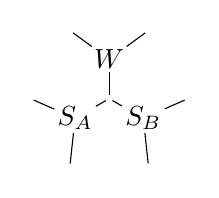
\begin{tikzpicture}[inner sep=1pt, baseline=.0em]
    \node (m) at (0,0) {$\sbullet$};
    \node (W) at (0,.5) {$W$};
    \node (SB) at (-30:.5) {$S_B$};
    \node (SA) at (-150:.5) {$S_A$};
    \node (w1) at (60:1) {};
    \node (w2) at (120:1) {};
    \node (sa1) at (-120:1) {};
    \node (sa2) at (-180:1) {};
    \node (sb1) at (-0:1) {};
    \node (sb2) at (-60:1) {};
    \draw (m) -- (W);
    \draw (m) -- (SA);
    \draw (m) -- (SB);
    \draw (W) -- (w1) {};
    \draw (W) -- (w2) {};
    \draw (SB) -- (sb1) {};
    \draw (SB) -- (sb2) {};
    \draw (SA) -- (sa1) {};
    \draw (SA) -- (sa2) {};
\end{tikzpicture}
=
\begin{tikzpicture}[inner sep=1pt, baseline=.0em]
    \node (m) at (0,0) {};
    \node (W) at (0,.5) {};
    \node (SB) at (-30:.5) {};
    \node (SA) at (-150:.5) {};
    \node (w1) at (60:1) {};
    \node (w2) at (120:1) {};
    \node (sa1) at (-120:1) {};
    \node (sa2) at (-180:1) {};
    \node (sb1) at (-0:1) {};
    \node (sb2) at (-60:1) {};
    \draw (sa2) .. controls (SA) and (W) .. (w2);
    \draw (sa1) .. controls (SA) and (SB) .. (sb2);
    \draw (sb1) .. controls (SB) and (W) .. (w1);
\end{tikzpicture}
.
\]
% TODO: This actually looks like one of the weird plots Penrose makes. Just without the `symmetrization'. Could it be relevant?
%We say that the tensor $I_2\otimes I_2\otimes I_2$ has rank 7, because it can be written as a sum of 7 simple tensors.
%
为了以快于通常 $n^3$ 时间的方式相乘两个矩阵 $A$ 和 $B$，
我们把它们重塑为形状为 $(2,\frac n 2,2,\frac n 2)$ 的块矩阵，并使用 Strassen 的张量：
%This means that if we have two $n\times n$ matrices, $A$ and $B$, and we write them as block matrices, shape $2\times \frac n2\times 2\times \frac n2$, we get
\[
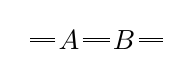
\begin{tikzpicture}[inner sep=1pt, baseline=.0em]
    \node (A) at (-.35, 0) {$A$};
    \node (B) at (.35, 0) {$B$};
    \draw[double] (B) -- ++(.5, 0) {};
    \draw[double] (A) -- ++(-.5, 0) {};
    \draw[double] (A) -- (B) {};
\end{tikzpicture}
=
\begin{tikzpicture}[inner sep=1pt, baseline=-1em]
    \node (m) at (0,0) {};
    \node (W) at (0,.4) {};
    \node (SB) at (-30:.5) {};
    \node (SA) at (-150:.5) {};
    \node (w1) at (.8, 0) {};
    \node (w2) at (-.8, 0) {};
    \node[below=.6em of SA] (A) {$A$};
    \node[below=.6em of SB] (B) {$B$};
    \draw (A) .. controls (-.75,-.5) and (0, 0) .. (w2);
    \draw (A) edge[out=50, in=130] (B);
    \draw (B) .. controls (.75, -.5) and (0, 0) .. (w1);
    \draw (B) -- ++(.5, 0) {};
    \draw (A) -- ++(-.5, 0) {};
    \draw (A) -- (B) {};
\end{tikzpicture}
=
\begin{tikzpicture}[inner sep=1pt, baseline=.0em]
    \node (m) at (0,0) {$\sbullet$};
    \node (W) at (0,.4) {$W$};
    \node (SB) at (-30:.5) {$S_B$};
    \node (SA) at (-150:.5) {$S_A$};
    \node (w1) at (60:1) {};
    \node (w2) at (120:1) {};
    \node (sa1) at (-120:1) {};
    \node (sa2) at (-180:1) {};
    \node (sb1) at (-0:1) {};
    \node (sb2) at (-60:1) {};
    \node[below=.6em of SA] (A) {$A$};
    \node[below=.6em of SB] (B) {$B$};
    \draw (m) -- (W);
    \draw (m) -- (SA);
    \draw (m) -- (SB);
    \draw (W) -- ++(1, 0) {};
    \draw (W) -- ++(-1, 0) {};
    \draw (SB) edge[bend left] (B) {};
    \draw (SB) edge[bend right] (B) {};
    \draw (SA) edge[bend left] (A) {};
    \draw (SA) edge[bend right] (A) {};
    \draw (B) -- ++(.5, 0) {};
    \draw (A) -- ++(-.5, 0) {};
    \draw (A) -- (B) {};
\end{tikzpicture}
.
\]
按正确顺序缩并这些边，只需要 $7/8 n^3 + O(n^2)$ 次运算。

如果改为重塑成 $(2,2,\dots,2)$，
\[
AB = 
   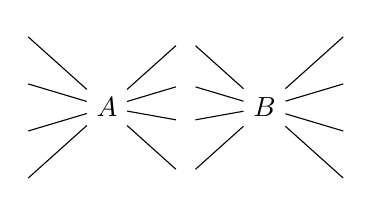
\begin{tikzpicture}[baseline=-1em, y=1.7em]
      \node (P1) at (0,-.5) {$A$};
      \node (A) at (1,1) {};
      \node (P2) at (2,-.5) {$B$};
      \node (B) at (1,0) {};
      \node (C) at (1,-.8) {};
      \node (D) at (1,-2) {};
      \draw (-1,1) -- (P1) -- (A) -- (P2) -- (3, 1);
      \draw (-1,0) -- (P1) -- (B) -- (P2) -- (3, 0);
      \draw (-1,-1) -- (P1) -- (C) -- (P2) -- (3, -1);
      \draw (-1,-2) -- (P1) -- (D) -- (P2) -- (3, -2);
   \end{tikzpicture}
   \,,
\]
并沿每个轴使用 Strassen 张量，那么工作量会减少 $(7/8)^{\log_2(n)}$，从而得到时间为 $n^{3 + \log_2(7/8)} = n^{2.80735}$ 的矩阵乘法。


\newpage

缩并双边 $S_A - A$ 和 $S_B - B$ 都需要 $O(n^2)$ 时间。

还需要验证这确实比朴素矩阵乘法更快：
缩并 $S_A - A$ 需要 $7\cdot 2^2 (n/2)^2$ 次运算，$S_B - B$ 同理。
接下来缩并 $S_AA - S_BB$，这需要 $7(n/2)^3$ 时间。
最后缩并与 $W$ 相连的边，需要 $2^2 \cdot 7 (n/2)^2$。
关键项是三次项 $7/8 n^3$；如果改为递归执行，就得到经典的 $O(n^{\log_2 7})$ 算法。

FIXME：什么是“与 $W$ 相连的边”？我认为我们必须/想要立即缩并与 $W$ 相连的超边？

\subsubsection{其他}

如果改用形状为 $(n,m)$ 和 $(m,p)$ 的块来表示 $A$ 和 $B$，就可以分解 $I_n\otimes I_m\otimes I_p$，并用与上面 Strassen $(2,2,2)$ 张量相同的方法得到矩阵乘法算法。
许多论文研究过这个问题，并由此产生了 Josh Alman 等人的最佳算法。
例如，Deep Mind 找到了 $I_3\otimes I_4\otimes I_5$ 的秩 47 分解。

也许更有趣的例子是 $(4,4,4)$ 张量，他们为它找到了一个秩 47 分解。
一种容易构造秩 49 分解的方法是取 Strassen 分解并把它加倍。
这会是一个值得展示的例子吗？也许太杂乱了？
不过实际上，他们的秩 47 构造只在“模”（modular）情形下成立。于是 $(3,4,5)$ 是一般情形。

